\chapter{Predicting flight delay}
In this chapter, the focus is moved on to prediction of flight delays using the historical flight dataset created. But before moving on to the actual prediction let's revisit the main aim of the predicting flight delays.
\\The work of underwriters in insurance industry is to decide the insurance payout rates. It is a complex process with many terms and conditions, and where consumer interest is not the first priority. The flight delay prediction will help in automating this whole process. Additionally, in a bid to be more transparent to the customer, the payout rates will be shown to the user before buying the insurance so that the user can take a better decision for themselves. The rates will be based on the probability of flights getting delayed. In simple terms, if the model predicts high probability of delay, the insurance payout will be lower. If the model predicts low probability of delay, the insurance payout will be higher.
\\There are two considerations that should be kept in mind as the reason for predicting the flight delays correctly.
\begin{enumerate}
    \item If the flight is predicted to be delayed, the insurance payouts will be lower for the flight. If a high number of flights are predicted wrongly as delayed, the consumers are going to see a lower payout rates for most of the flights. This will reduce the consumer interest in the platform.
    \item If the flight is predicted to be on-time, the insurance payouts will be higher for the flight. If a high number of flights are predicted wrongly as on-time, the consumers are going to see a high payout rates for most of the flights. This will be a loss-making proposition for the platform so should be avoided.
\end{enumerate}

\section{Exploratory Data Analysis}
It's a good idea to look at the dataset before starting the prediction. Some of the relations between variables are discovered through exploratory data analysis and it will help in setting the direction for data analysis.
\\The first relationship to focus on is the average delays at the airports as well as airlines. For sake of clarity, only top eight airlines are chosen. 

\begin{figure*}[h]
    \centering
    \begin{subfigure}[h]{0.5\textwidth}
        \centering
        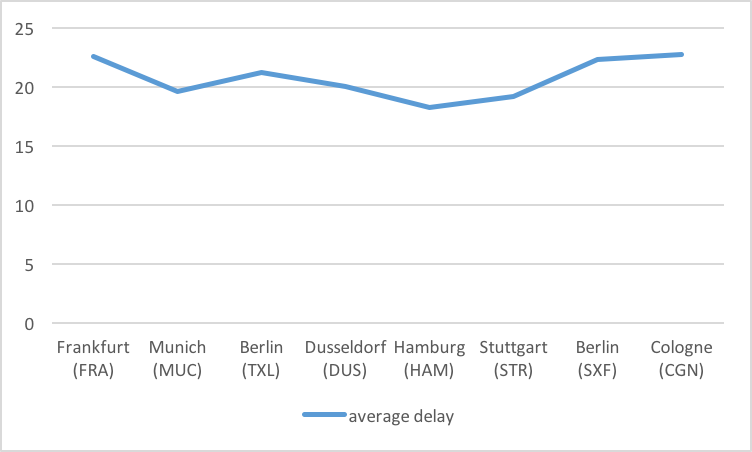
\includegraphics[height=1.7in]{Figures/airport_delay.png}
        \caption{Average delay at top destination airports}
    \end{subfigure}%
    ~ 
    \begin{subfigure}[h]{0.5\textwidth}
        \centering
        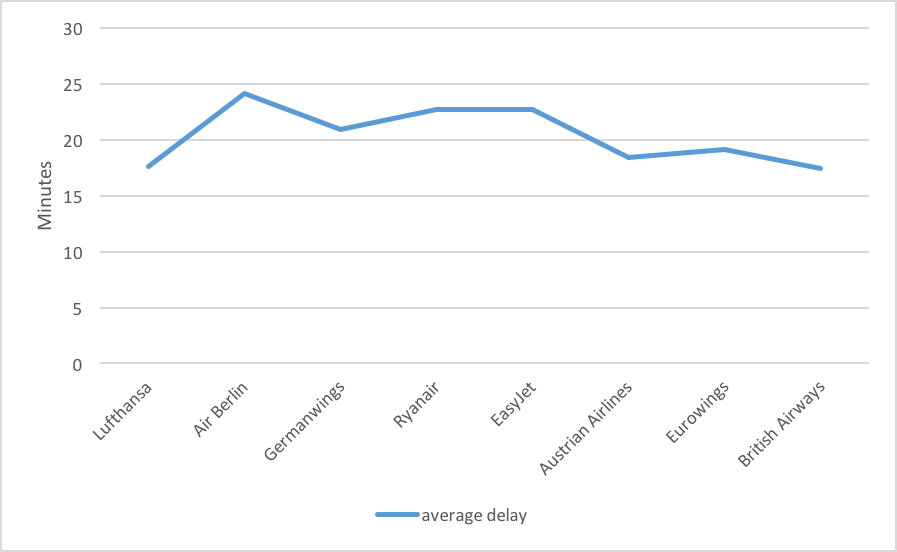
\includegraphics[height=1.7in]{Figures/airline_delay.png}
        \caption{Average delay of top airlines}
    \end{subfigure}
    \caption{Average delay in minutes}
\end{figure*}

Next important consideration is the ratio of delayed flights to flights on time. In the figures, the ratio can be seen for top 8 airlines as well as airports

\begin{figure*}[h]
    \centering
    \begin{subfigure}[h]{0.5\textwidth}
        \centering
        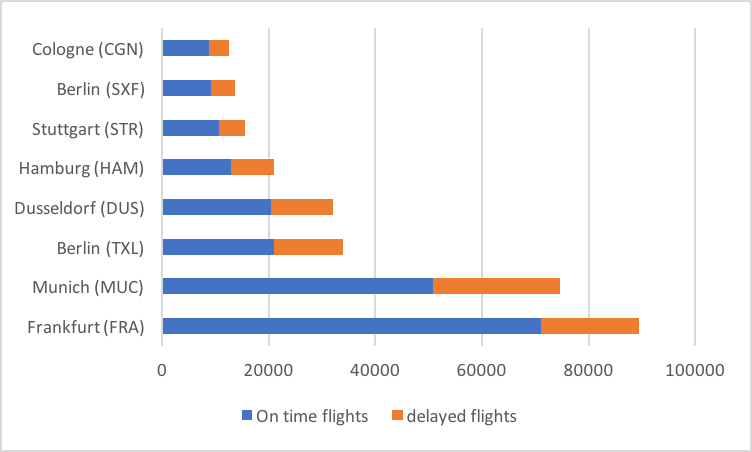
\includegraphics[height=1.7in]{Figures/airport_delay_ratio.png}
        \caption{Delayed flights vs On-time flights for top airlines}
    \end{subfigure}%
    ~ 
    \begin{subfigure}[h]{0.5\textwidth}
        \centering
        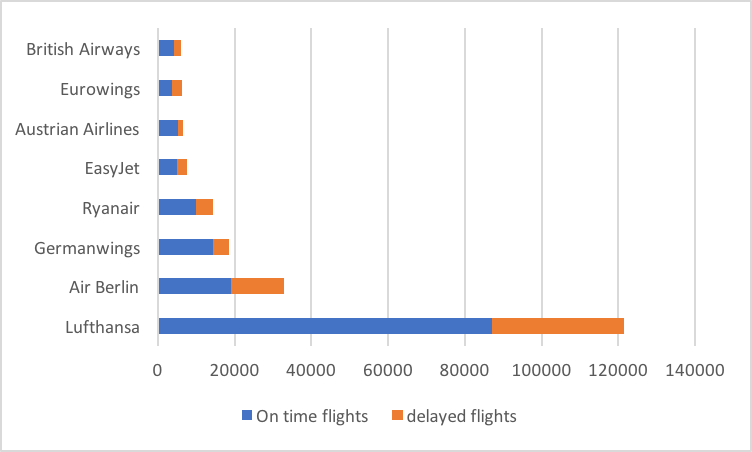
\includegraphics[height=1.7in]{Figures/airline_delay_ratio.png}
        \caption{Delayed flights vs On-time flights for top airlines}
    \end{subfigure}
    \caption{Delayed flights vs On-time flights}
\end{figure*}


\section{Prediction}
The prediction techniques can be classified into two categories, classification and regression. As already mentioned, the target variable for the desired model would contain 4 prediction classes. The classification algorithms directly classify predicted delay to these four classes. The regression technique on the other hand predicts flight delay in minutes. Using the predicted minutes, the flight delay classes will be decided.

\subsection{Implementation}
All the algorithms were first tested using RStudio in R language. For testing different prediction algorithms, the dataset was divided into a training and test dataset. Training set was 75\% of the whole dataset and the test set was the remaining 25\%. The algorithm finalised was implemented in python for real time prediction of flight delays on the web platform.

\subsection{Confusion matrix}
The accuracy of any prediction model can be measured by prediction error. But in this case, there is a very large number of flights that are not delayed (>80\%). If the model predicts all flights as not delayed, the accuracy will be >80\%, a very good prediction normally, but what is clearly deceiving in this particular case. Due to this predicament, each model was evaluated using confusion matrix. Confusion matrix is often used to describe the performance of classification model. It is a table showing the actual values in rows and how they were predicted by the model, mentioned in columns. 
%\begin{figure}[H]
%    \centering
%    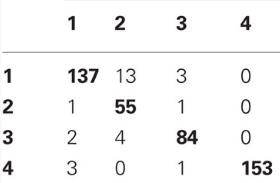
\includegraphics[]{Figures/confusion_matrix_ex.png}
%    \caption{Example of a confusion matrix}
%    \label{fig:confusion_matrix_ex}
%\end{figure}

\begin{wrapfigure}{R}{0.5\textwidth} 
\vspace{-20pt}
  \begin{center}
    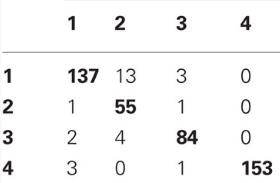
\includegraphics[width=0.4\textwidth]{Figures/confusion_matrix_ex.png}
    \caption{Example of a confusion matrix}
    \label{fig:confusion_matrix_ex}
  \end{center}
  \vspace{-20pt}
  \vspace{1pt}
\end{wrapfigure} 

As seen in figure \ref{fig:confusion_matrix_ex}, the rows are the actual values and the columns are the predicted values. Taking the first row as context, the actual value is 1. 137 is the number of values predicted correctly as 1. 13 is the number of values where the correct prediction was 1 but the model predicted 2, and so on. In essence, the diagonal values of a confusion matrix are the correct predictions, and the model's aim will be to increase the diagonal values.

\section{Prediction using Classification}
In statistics, classification is the problem of identifying to which of a set of categories does a new observation belong to. An example would be assigning a given object into "sphere" or "non-sphere" classes or assigning a piece of code as "virus", "suspicious" or "not virus" based on certain characteristics of the operations the code performs.
\\An algorithm that implements classification is known as a classifier. These classifiers are further divided into binary classifiers, those that classify to only two classes, and multiclass algorithms, the ones which will be used for this dataset.

\subsection{Random Forest}
Random forest is an ensemble learning method for classification (and regression) that operates by constructing a multitude of decision trees at training time and outputting the class that is the mode(value that appears most often) of the classes output by individual trees.\cite{TinKamHoRandomForests}
It is an improvement of decision trees algorithm, which had a habit of overfitting to their training set\cite{Winham2013APerformance}.
\\There are multiple packages that implement random forest in R, the most famous being \textit{randomForest}. But instead the package used for this model is called \textit{ranger}. The latter is used because it exploits the full potential of a multiclass architecture and is much faster than the original implementation. Starting with the predictions, with default parameters, and running with a count of 100 trees, the confusion matrix calculated is as shown in table \ref{table:cm_rf_100}.

\begin{table}[H]
\centering
\begin{tabular}{l | a | b | a | b | a}
\hline
\rowcolor{LightCyan}
\mc{1}{Actual Delay class}  & \mc{1}{Class 0} & \mc{1}{Class 1} & \mc{1}{Class 2} & \mc{1}{Class 3} & \mc{1}{Grand Total} \\
\hline
Class 0 & 71066 & 565 & 35 & 11 & 71677 \\
Class 1 & 6920 & 1280 & 41 & 4 & 8245\\ 
Class 2 & 962 & 168 & 168 & 1 & 1299\\
Class 3 & 322 & 25 & 16 & 58 & 421\\ \hline
Grand Total & 79270 & 2038 & 260 & 74 & 81642
\end{tabular}
\caption{Classification using Random Forest, 100 trees}
\label{table:cm_rf_100}
\end{table}

As this is the first confusion matrix calculated, it's prudent that it should be discussed in detail. The ensuing ones won't be discussed in such detail.
\\With a test set of about 81000 flights among which 71694 flights were on time, the model correctly predicts no delay(class 0) for 71066 flights. Among those incorrectly predicted as not delayed, 565 were classified as class 1(delay less than an hour), 35 were classified as class 2(delayed more than an hour) and 11 were classified as class 3 (delayed more than 2 hours). 
\\Now let's go through row of class 2. These belong to flights that were delayed for more than an hour. The correct flights predicted with class 2 were 168, whereas 962 flights were declared as not-delayed. This behaviour can be seen for all delay classes. The prediction models overwhelmingly classify flights as not delayed even though they were delayed. The next step is to optimise the model to improve the prediction of flights actually delayed.

Optimising the random forest parameters is possible using the \textit{caret} package. The algorithm was optimised using the code as follows

\begin{lstlisting}[language=R, breaklines=true]
tr <- trainControl(method = "cv", number = 5)
train( train\$flight_delay_bins ~ .,data=train,method="rf",trControl= tr)
\end{lstlisting}

The output of the optimisation process using cross validation among multiple random forest models was that the variable \textit{mtry} should be set to 3. It is the number of variables available for splitting at each tree node. Further explanation for the variable is out of scope of the Thesis. For each of the following models, \textit{mtry} was kept to 3. The next way to optimise the algorithm was using different number of trees for the algorithm. The result is as follows.


\begin{table}[H]
\centering
\begin{tabular}{l | a | b | a | b | a}
\hline
\rowcolor{LightCyan}
\mc{1}{Actual Delay class}  & \mc{1}{Class 0} & \mc{1}{Class 1} & \mc{1}{Class 2} & \mc{1}{Class 3} & \mc{1}{Grand Total} \\
\hline
Class 0 & 71018 & 608 & 38 & 13 & 71677 \\
Class 1 & 6902 & 1294 & 43 & 6 & 8245\\ 
Class 2 & 976 & 163 & 160 & 0 & 1299\\
Class 3 & 323 & 22 & 17 & 58 & 59\\ \hline
Grand Total & 79219 & 2087 & 258 & 78 & 81642
\end{tabular}
\caption{Classification using Random Forest, 50 trees}
\label{table:rf_50_no_w}
\end{table}


\begin{table}[H]
\centering
\begin{tabular}{l | a | b | a | b | a}
\hline
\rowcolor{LightCyan}
\mc{1}{Actual Delay class}  & \mc{1}{Class 0} & \mc{1}{Class 1} & \mc{1}{Class 2} & \mc{1}{Class 3} & \mc{1}{Grand Total} \\
\hline
Class 0 & 71101 & 532 & 31 & 13 & 71677 \\
Class 1 & 6896 & 1301 & 44 & 4 & 8245\\ 
Class 2 & 973 & 159 & 167 & 0 & 1299\\
Class 3 & 320 & 23 & 19 & 59 & 421\\ \hline
Grand Total & 79290 & 2015 & 261 & 76 & 81642
\end{tabular}
\caption{Classification using Random Forest, 200 trees}
\label{table:rf_200_no_w}
\end{table}

As can be observed, increasing the number of trees didn't result in any reasonable improvements. Further strategies were required to improve the model.

\subsubsection{Adding new variables to improve performance}
Recalling the point made in the Flight data chapter, the departure airports were removed from the prediction dataset as that variable had over 200 unique values, or factors. The reasonable limit for the number of factors was to be kept till 32, the random forest classifier's limit. Hence instead of using different airports, it was decided to use countries instead. Mapping departure airports to countries resulted in 86 unique values. This variable still had too many factors, so the lowest 54 countries were combined into one value called "Other" as shown in table \ref{fig:other_country}

\begin{figure}[H]
    \centering
    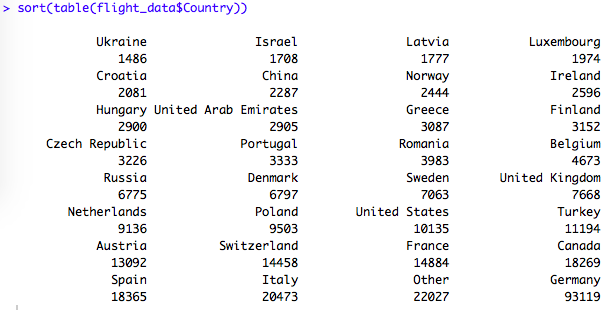
\includegraphics[width=\textwidth]{Figures/other_country.png}
    \caption{Departure flights mapped to countries}
    \label{fig:other_country}
\end{figure}


%\begin{table}[H]
%\centering
%\begin{tabular}{||c c||} 
%\hline
%Country & Frequency  \\ [0.5ex] 
%\hline\hline
%Ukraine  &  1486 \\
%Israel  &  1708 \\
%Latvia  &  1777 \\
%Luxembourg  &  1974 \\
%Croatia  &  2081 \\
%China  &  2287 \\
%5Norway  &  2444 \\
%Ireland  &  2596 \\
%Hungary  &  2900 \\
%United Arab Emirates  &  2905 \\
%Greece   & 3087 \\
%Finland  &  3152 \\
%Czech Republic  &  3226 \\
%Portugal  &  3333 \\
%Romania  &  3983 \\
%Belgium  &  4673 \\
%ussia  &  6775 \\
%Denmark  &  6797 \\
%Sweden  &  7063 \\
%United Kingdom  &  7668 \\
%Netherlands  &  9136 \\
%Poland  &  9503 \\
%United States &  10135 \\
%Turkey &  11194 \\
%Austria  & 13092 \\
%Switzerland  & 14458 \\
%rance &  14884 \\
%Canada &  18269 \\
%Spain &  18365 \\
%Italy &  20473 \\
%Other &  22027 \\
%Germany  & 93119\\
%\hline \hline
%\end{tabular}
%\caption{Departure flights mapped to countries}
%\label{table:other_country}
%\end{table}

Adding the variable to our dataset though didn't improve the prediction much but it did slightly increase the correct prediction of class 2 and 3 as can be seen in figure \ref{table:rf_with_country}

\begin{table}[H]
\centering
\begin{tabular}{l | a | b | a | b | a}
\hline
\rowcolor{LightCyan}
\mc{1}{Actual Delay class}  & \mc{1}{Class 0} & \mc{1}{Class 1} & \mc{1}{Class 2} & \mc{1}{Class 3} & \mc{1}{Grand Total} \\
\hline
Class 0 & 71290 & 365 & 14 & 8 & 71677 \\
Class 1 & 6976 & 1214 & 50 & 5 & 8245\\ 
Class 2 & 976 & 160 & 159 & 4 & 1299\\
Class 3 & 332 & 13 & 11 & 65 & 421\\ \hline
Grand Total & 79574 & 1752 & 234 & 82 & 81642
\end{tabular}
\caption{Confusion matrix of random forest with added country variable}
\label{table:rf_with_country}
\end{table}

\subsection{XGBoost}
XGBoost is an optimised distributed gradient boosting library designed to be highly efficient, flexible and portable. It implements machine learning algorithms under the Gradient Boosting framework. These optimisations result in making XGBoost highly scalable for large amount of data, using far fewer resources than existing systems.\cite{Chen2016XGBoost:System}
Gradient boosting of regression trees produces competitive, highly robust, interpretable procedures for both regression and classification, especially appropriate for mining less than clean data. \cite{Hastie2001TheIllustrations} Using XGBoost meant that all factor variable be converted to indicator columns and dataset saved as a matrix and passed on to the model. The multiclass classification algorithm of XGBoost provides probability of each class instead of predicting the actual class. The prediction after 200 rounds was as follows.




\section{Fixing class imbalance problems}
The prediction error up till now has been hovering at about 15\%. But the absolute error in this case is misleading. As the number of flights which were on time is much larger than the number of flights that got delayed, even classifying every flight as not delayed will give an error rate of about 15\% in our dataset. This is known as class imbalance problem and needs to be fixed. One way of fixing the issue is giving weights to different classes based on the frequency of the class. In simple terms, the class with the highest frequency will be given the lowest weight whereas the class with lowest frequency will be given the highest weight. The class imbalance issue was tried to be fixed using both XGBoost and randomforest algorithms.

\subsection{XGBoost}
XGBoost natively supports fixing class imbalance problem. It has a variable called \textit{scale\_pos\_weight} that is used to give weight to classes. But this value does not accept a vector. Instead it is just a value that is used as a weight for the positive class (in our case, the flight delayed class). This variable, by design, just works with binary classification. Even when tried for multiclass classification, the trained model just predicts the test dataset in binary as seen in table \ref{table:xgboost_w} .
\begin{table}[H]
\centering
\begin{tabular}{l | a | b | a}
\hline
\rowcolor{LightCyan}
\mc{1}{Actual Delay class}  & \mc{1}{Class 0} & \mc{1}{Class 1} & \mc{1}{Grand Total} \\
\hline
Class 0 & 32866 & 10946 & 43812 \\
Class 1 & 3879 & 1217 & 5096\\ 
Class 2 & 602 & 186 &  788\\
Class 3 & 219 & 77 & 296\\ \hline
Grand Total & 37566 & 12426 & 49992
\end{tabular}
\caption{XGBoost just predicts 1 or 0 if using scale\_pos\_weight}
\label{table:xgboost_w}
\end{table}
The other way to improve class imbalance problem was to use the evaluation metric as AUC, or Area under ROC curve. In an ROC curve the true positive rate (flights correctly predicted as delayed) is plotted in function of the false positive rate(flights incorrectly predicted as delayed). Instead of improving on basis of reducing absolute error, XGBoost instead tries to maximise area under ROC curve. But unfortunately, for multiclass classification, XGBoost doesn't allow AUC as an evaluation metric. Consequently the idea of fixing class imbalance problem using XGBoost was dropped.


\subsection{Using Random Forest}
Similar to most classifiers, Random Forest can also suffer from the curse of learning from an extremely imbalanced training data set. As it is constructed to minimise the overall error rate, it will tend to focus more on the prediction accuracy of the majority class, which often results in poor accuracy for the minority class.\cite{Chen2004UsingDatab}. In Random forest, the weight signifies the probability an observation is selected for the tree. Observations with higher weights are selected more frequently. The same package for Random Forest, \textit{ranger} will now be used with weights. This package expects a vector with the same length of the number of observations in the dataset. The weights were calculated on the basis of the frequency of classes. The weighted model didn't give any tangible improvements when the weight was calculated on the basis of inverse of frequency of classes. It was decided the ratio of weights should be even more amplified. A multitude of different weights were calculated but the one that gave the best result was this. 
    
\begin{lstlisting}[language=R, breaklines=true]
weights <- NULL
weights <- ifelse(train\$flight_delay_bins == "0", (1/table(train\$flight_delay_bins)[1]) * 0.10, 0)
weights <- ifelse(train\$flight_delay_bins == "1", (1/table(train\$flight_delay_bins)[2]) * 0.20, weights)
weights <- ifelse(train\$flight_delay_bins == "2", (1/table(train\$flight_delay_bins)[3]) * 0.30 , weights)
weights <- ifelse(train\$flight_delay_bins == "3", (1/table(train\$flight_delay_bins)[4]) * 0.40, weights)
\end{lstlisting}

This weight variable, finalised as a result of many trial and error, along with number of trees increased to 200, resulted in a marked improvement over the test prediction dataset. The confusion matrix, table \ref{table:rf_100_w}, has all it's diagonal elements maximised compared to the other results. In class 3, even though more classes are predicted as class 1, it is considered acceptable as more flights are still classified as delayed rather than on-time. This is the ideal prediction desired for the project's requirement.


\begin{table}[H]
\centering
\begin{tabular}{l | a | b | a | b | a}
\hline
\rowcolor{LightCyan}
\mc{1}{Actual Delay class}  & \mc{1}{Class 0} & \mc{1}{Class 1} & \mc{1}{Class 2} & \mc{1}{Class 3} & \mc{1}{Grand Total} \\
\hline
Class 0 & 53710 & 17430 & 396 & 141 & 71677 \\
Class 1 & 2997 & 5054 & 168 & 26 & 8245\\ 
Class 2 & 348 & 706 & 235 & 10 & 1299\\
Class 3 & 123 & 185 & 30 & 83 & 421\\ \hline
Grand Total & 57178 & 23375 & 829 & 260 & 81642
\end{tabular}
\caption{Random forest with weighted variable}
\label{table:rf_100_w}
\end{table}

\section{Prediction using regression}
Even though a good prediction was achieved using classification with weights, regression was also tested to see if it could preform better. In statistical modelling, regression is defined as the process to evaluate degree of relationship among the data variables. For the platform, the target variable for regression model is arrival delay in seconds.

\subsection{Linear Modelling}
Beginning with the basics, the first algorithm chosen for regression was linear modelling using R function called \textit{lm}. Unfortunately the result of the model wasn't satisfactory. The adjusted R-squared value of the model was just .1272. A good result has an r squared value much closer to 1. As the result was so far from ideal, it was not considered for further improvements.

\subsection{Random Forest}
Random forest, already used as a classification algorithm, can also be used for a regression model. Using default parameters, and the target variable as arrival delay, the R-squared of the algorithm comes up to be .1319, as seen in figure \ref{fig:regression_rf_no_departure}. Again, this is not an ideal result. As both the results of the regression were terrible, the idea of prediction using regression was dropped.

\begin{figure}[h]
    \centering
    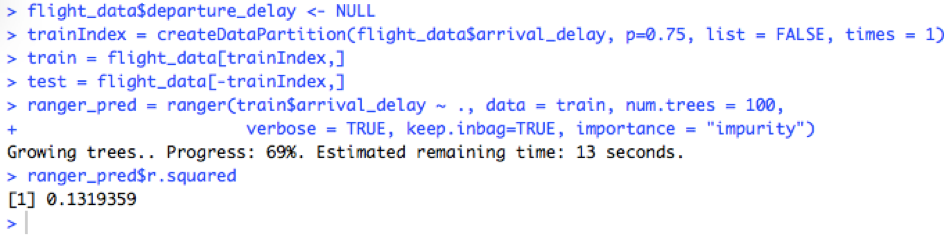
\includegraphics[width=\textwidth]{Figures/regression_rf_no_departure.png}
    \caption{Regression using Random Forest}
    \label{fig:regression_rf_no_departure}
\end{figure}

There is one thing to note that if the variable departure delay is used in the dataset, the predictions improve dramatically. The R-squared value for random forest improves from .13 to .86. Unfortunately it can't be used as this variable won't be available while predicting the flight delays for future flights.

\begin{figure}[h]
    \centering
    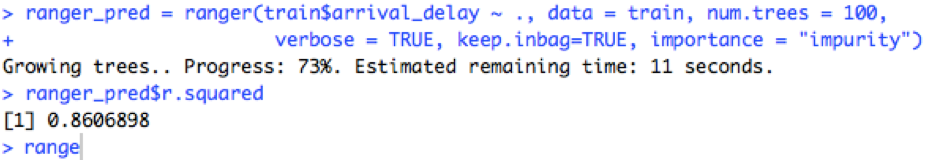
\includegraphics[width=\textwidth]{Figures/regression_rf.png}
    \caption{Regression using Random Forest, including departure delay}
    \label{fig:regression_rf}
\end{figure}


\section{Conclusion}
Based on the analysis done so far, the class imbalance problem was fixed to a large extent via using weights with random forest algorithm. Even though the absolute accuracy of the model decreases if using weights, this model is more suitable to the problem at hand.